\chapter{Theoretical Background of Survey Modelling}
\label{ch:surveymodelling}

Space missions are very expensive to design, build, launch and operate. Therefore, it is important that all properties and behaviors of such a mission are well known in advance. Then, an accurate assessment can be made of the merits of the mission and what results are to be expected. In addition, it allows for selecting the design which will produce the best results. In order to study these properties and determine the optimum, computer simulations are an excellent tool. They allow for cheap and rapid testing of a multitude of possible mission parameters, and recording the relevant data for easy analysis. \\

Currently, no model is publicly available for modelling multi-spacecraft surveys. Therefore, a simulation will be developed. During and after development, the model is also extensively verified and validated. The process for this is described in \autoref{ch:vandv}. Other research (e.g. \cite{Flyeye}, \cite{2017NEOSDT}) has demonstrated the potential for explicitly modelling the entire survey as it would be conducted by the actual system. In this chapter, the theoretical background from sources in literature for the various steps in simulating a NEA survey will be given. Implementation of the simulation will then be treated in the next chapter: the contents of this chapter are all sourced from literature.\\

The components of the simulation consist of first generating a representative population of asteroids (described in \autoref{sec:modelling_population}), then, at each timestep, calculating the background and target signal (\autoref{sec:modelling_background} and \autoref{sec:modelling_target}, respectively). Knowing these signals, the signal-to-noise ratios can then be determined after estimation of some of the detector properties (\autoref{sec:modelling_hardware_SNR}). The frequency and location of the observations is determined by the search strategy, and resulting cadence (detailed in \autoref{sec:modelling_cadence}) and lastly through repeat observations, it can be determined whether the system is capable of identifying a target (\autoref{sec:modelling_identification}).\\

\section{Population of Asteroids}
\label{sec:modelling_population}
The first component of the simulation is the asteroid population model. This population was already briefly described in \autoref{sec:introduction_NEA}. In this section, more details on the generation of the population and the process of determining the positions of the NEAs, are given. As already mentioned in \autoref{sec:introduction_NEA}, the most comprehensive debiased population model is the one by \cite{GranvikPopulation}. This population model was generated by propagating an initial population of NEAs based on several known interactions (e.g. gravitational interaction with the planets), and then comparing the resulting population to the results of the NEOWISE mission. Essentially, the problem then reduces to the question: ``What initial population would result in the results that are observed in the NEOWISE mission?''. Then, the initial population model can be fitted to the results of the NEOWISE mission, and a debiased population model is thus obtained. \\

\begin{figure}[htbp]
 \centering
 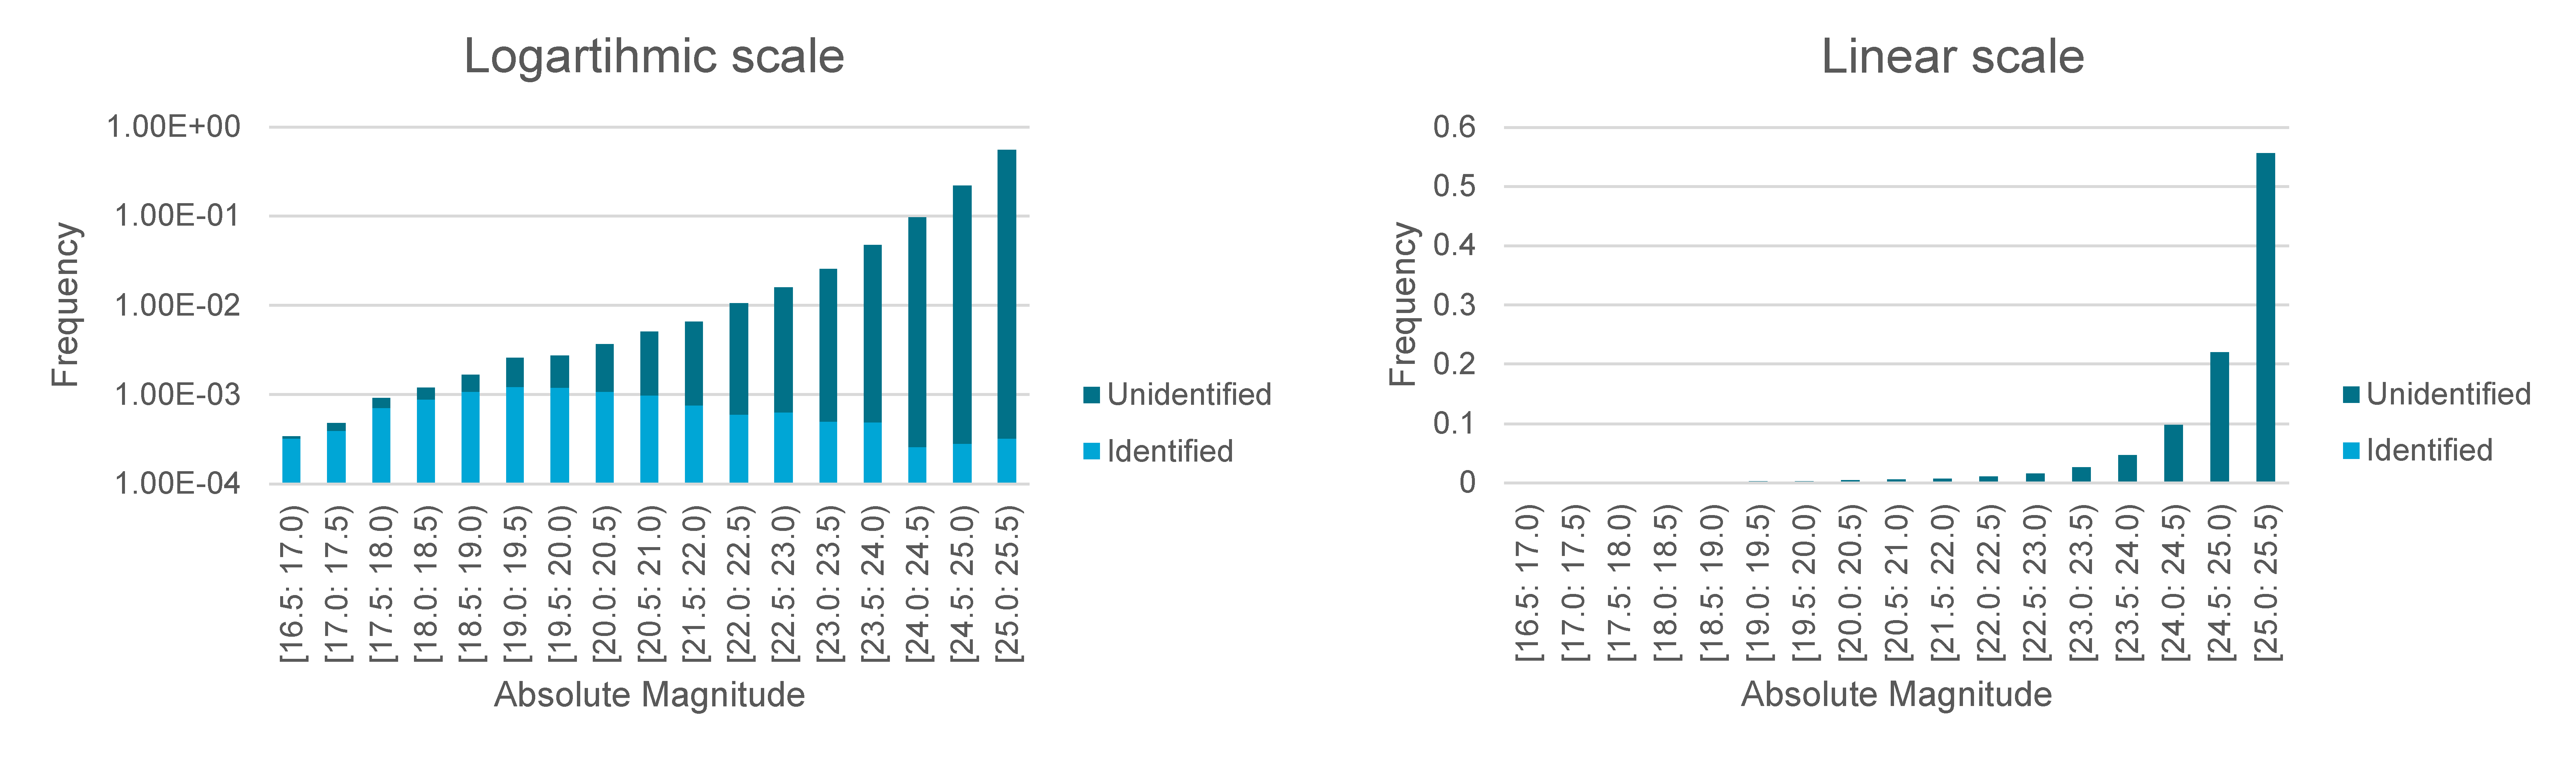
\includegraphics[width=1.0\textwidth]{img/population_identification_correction.pdf}
 \caption{Distribution of the full population of asteroids per \cite{GranvikPopulation}, and an estimation of how many asteroids have already been identified, per \cite{HarrisPopulation}. The left graph is shown logarithmically, the right graph uses a linear scaling.}
 \label{fig:populationcorrection}
\end{figure}


Of course, this results in a full population of NEAs; whereas a population of \textit{unidentified} NEAs is required for this work. Therefore, a correction to the population was made based on the work of \cite{HarrisPopulation}. To do this, the population as given by \cite{GranvikPopulation} was separated, based on absolute magnitude, into bins of width 0.5. Then, it was assumed that the detection of NEAs is roughly uniform over the orbital parameters. The completeness statistics of \cite{HarrisPopulation} can then be used to discard a part of the population as \textit{identified}. For example, assume there are 1000 asteroids in the $H=(21.0; 21.5]$ absolute magnitude bin. \cite{HarrisPopulation} predicts a completeness of 0.115 for this range. Thus, to correct for the known fraction of NEAs, 115 out of the 1000 asteroids are selected randomly, and removed from the population. This process is performed for every absolute magnitude bin between $H=16.5$ and $H=25.5$. The result of this process is shown in \autoref{fig:populationcorrection}. Of course, the assumption of uniformity in the detection of NEAs is false: highly eccentric NEAs, NEAs that are very dark, or NEAs with a large semi-major axis are more likely to be undetected. However, no data is available on this matter, and therefore no better alternative was deemed to be available. The error is judged to be sufficiently small: firstly, all simulations will be affected equally. Secondly, as can be seen in the second diagram in \autoref{fig:populationcorrection}, only a small part of asteroids is discarded as the largest population groups by size have very low completeness numbers.

\section{Background Signal}
\label{sec:modelling_background}
Before considering the existing knowledge on modelling asteroid signals, first the background in which these targets has to be observed is discussed. In this section, the current relevant body of knowledge on modelling this background signal will be given. The background signal will be split into two components. Firstly, the background light originating from the Sun. This manifests most dramatically in the form of direct sunlight. However, also reflections off of interplantary dust are important. This reflection manifests in the phenomena of zodiacal light and gegenschein. The second component of the background signal, is the light from outside the Solar system. This light originates from other stars and manifests mainly as a diffuse background of starlight. Particularly, a very large concentration of this starlight is found around the galactic plane. \\

\begin{figure}[htbp]
 \centering
 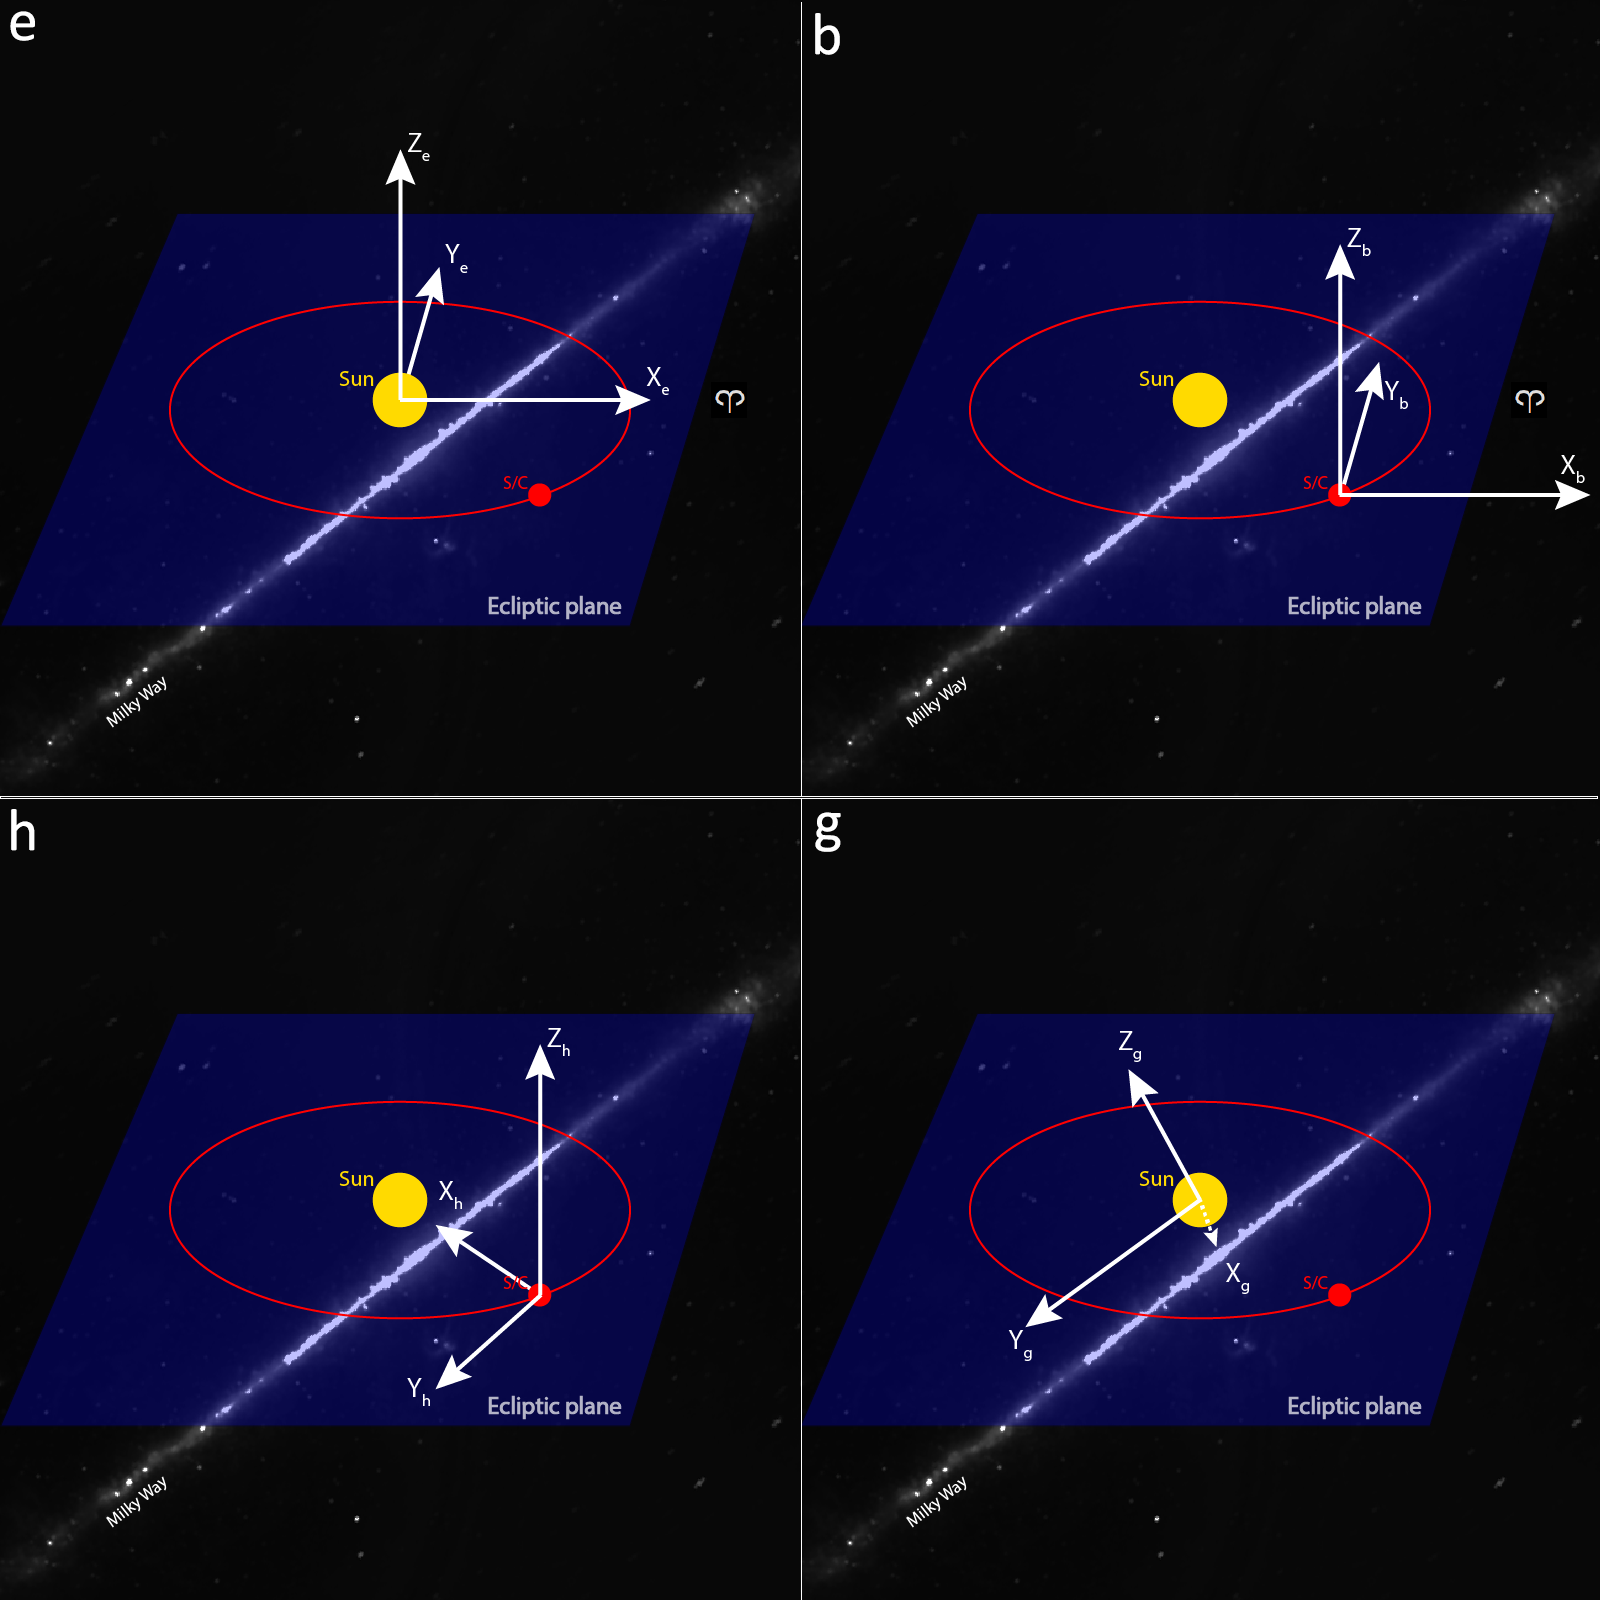
\includegraphics[width=1.0\textwidth]{img/referenceframes.png}
 \caption{Illustration of the utilized reference frames. Also shown are the Sun, spacecraft, ecliptic plane (incl. vernal equinox), and Milky Way.}
 \label{fig:referenceillustration}
\end{figure}


The reason for separating the background signal into these two components is straightforward: in a reference frame fixed among the stars, the background signal from outside the Solar system is practically unchanging as the spacecraft moves around the Sun; the parallax of moving several AU is negligible on galactic scales. In constrast, the contribution of light from our Sun is directly dependent on the position of the spacecraft with regards to the Sun. For the mathematical treatment of these signals, four reference frames are defined, which can be seen in \autoref{fig:referenceillustration}:

\newpage

\begin{itemize}
 \item \textbf{A heliocentric ecliptic reference frame} $e$: A right-handed reference frame whose principal plane is the ecliptic plane, origin at the center of the Sun, and the positive $X_e$-direction towards the vernal equinox.
 \item \textbf{A body-centered ecliptic reference frame} $b$: A right-handed reference frame whose principal plane is the orbital plane of the spacecraft, origin at the center of the spacecraft, and the positive $X_b$-direction towards the vernal equinox. Note that all orbits considered for the spacecraft lie in the ecliptic plane, and therefore this reference frame also has the ecliptic plane as its principal plane.
 \item \textbf{A body-centered ecliptic reference frame, oriented relative to the Sun} $h$: A right-handed reference frame defined similar to $b$, but with the positive $X_h$-direction towards the center of the Sun.
 \item \textbf{A galactic reference frame} $g$: A right-handed reference frame whose principal plane is the plane of the Milky Way, origin at the center of the Sun, and positive $X_g$-direction towards the galactic core.
\end{itemize}


The transformations between heliocentric ecliptic longitude and latitude $(l_e, b_e)$ and galactic longitude and latitude $(l_g, b_g)$ involve a series of rotations, and therefore require some reference values. With $b_{NGP}$ the latitude of the North Galactic Pole, approximately equal to $29.81^\circ$ or $0.5203 \mathrm{rad}$; ascending node of the Galaxy $l_{NGP}$, approximately $270.02^\circ$, $4.712 \mathrm{rad}$; and longitude of the galactic core $l_{GC}$, approximately $6.38^\circ$, or $0.1114 \mathrm{rad}$ (\cite{SkyBrightness}), the transformations are given by \cite{SkyBrightness} as follows:

\begin{align}
 b_g &= \sin ^{-1} (\sin b_e * \sin b_{NGP}) - \cos b_e \sin b_{NGP} \sin (l_e - l_{NGP}) \\
 \sin l_g' &= \frac{\sin b_e \cos b_{NGP} + \cos b_e \sin b_{NGP} \sin (l_e - l_{NGP})}{\cos b_g} \\
 \cos l_g' &= \frac{\cos (l_e - l_{NGP}) \cos b_e}{\cos b_g} \\
 l_g &= \begin{cases}
        \sin ^{-1} (\sin l_g') + l_{GC}; & \cos l_g' \geq 0 \\
        \pi - \sin^{-1} (\sin l_g') + l_{GC}; & \cos l_g' < 0, \sin l_g' > 0 \\
        - \pi - \sin^{-1} (\sin l_g') + l_{GC}; & \cos l_g' < 0, \sin l_g' \leq 0
       \end{cases}
\end{align}

The transformation from the $e$ to the $b$ frame is simply a translation by the spacecraft coordinates $[x_e^{S/C}, y_e^{S/C}, z_e^{S/C}]$:
\begin{align}
 x_b &= x_e - x_e^{S/C} \\
 y_b &= y_e - y_e^{S/C} \\
 z_b &= z_e - z_e^{S/C}
\end{align}

Where $z_e^{S/C}$ will generally be zero as the spacecraft is located in the ecliptic plane. As the values of $[x_e^{S/C}, y_e^{S/C}, z_e^{S/C}]$ are negligible on galactic scales, the transformations from the spacecraft-fixed frame $b$ to the galactic frame $g$ are the same as the transformation from the heliocentric frame $h$ to the galactic frame. Lastly, the transformation from the body-centered frame $b$, to the body-centered frame oriented relative to the Sun $h$, involves a rotation around the $Z_b$-axis. As the latitude of the Sun in the $b$-frame is zero, the transformation is simply a subtraction of the longitude of the Sun in the $b$-frame, $b_b^{\odot}$, from the longitude in the $b$-frame:
\begin{align}
 l_h &= l_b \\
 b_h &= b_b - b_b^{\odot}
\end{align}

With the reference frames defined, the individual components can be discussed. Firstly, the contribution of the Sun will be discussed, and then the background starlight for both thermal infrared and visual light.

\subsection{Solar contribution}
Modelling of the thermal infrared background radiation as a result of the light from the Sun is described by \cite{IRDust}, based on observations of the COBE mission. This model focusses on a modelling of the thermal state of interplanetary dust, and the resulting thermal infrared emission observed. Thus, the signal is not comprised of light originating at the Sun - but rather on the radiation from bodies heated by that light. The authors state that the albedo of particles at the relevant wavelengths is very close to zero, and therefore scattered Sunlight needs not be considered; only the emissions of the particles. Thus, the zodiacal flux $Z(l, b)$ can be expresssed as an integral over the line of sight (in practice, a distance up approximately the orbit of Jupiter is sufficient) of the sensor of the various contributions (which will be discussed in  more detail below):
\begin{equation}
 Z(l, b) = \Sigma_c \int _{\lambda_0} ^{\lambda_1} \int _S n_{c}(X, Y, Z)  E_{c}(\lambda) B(\lambda, T) ds d\lambda
 \label{eq:irdustflux}
\end{equation}
With $n_c$ the density of the dust due to a contribution $c$, $B$ is the blackbody emission given by Planck's law and $E_c$ is a wavelength-specific emission correction factor. The temperature of the dust grains is assumed to follow a power law function of distance from the Sun $R$:
\begin{equation}
 T(R) = T_0R^{-0.467}
\end{equation}
Temperature $T_0$ at 1 AU is set to $286\mathrm{K}$, and the emissivity modifications at the $4.9 \mu\mathrm{m}$ and $12 \mu\mathrm{m}$ thermal infrared wavelength are $0.997$ and $0.958$, respectively. Then, based on observations of the COBE mission, the authors construct a parametric model, based on three contributions. The first contribution is a ``donut-shaped'' dust cloud centered at the Sun, and inclined $2.03^\circ$ with respect to the ecliptic. This is the largest contributor to the density of interplanetary dust. Two more contributions which are modelled are a set of three dust bands, inclined at $0.56^\circ$, $1.2^\circ$ and $0.8^\circ$. Lastly, a circumsolar ring is modelled along the orbit of the Earth, which has a higher concentration around $10^\circ$ behind Earth in its orbit, as dust trails the planet due to its gravity. For conciseness, the exact model will not be described here in detail; interested readers can refer to \cite{IRDust}. An illustration of the contours of the components is seen in \autoref{fig:irdustcontributions}.\\

\begin{figure}[htbp]
 \centering
 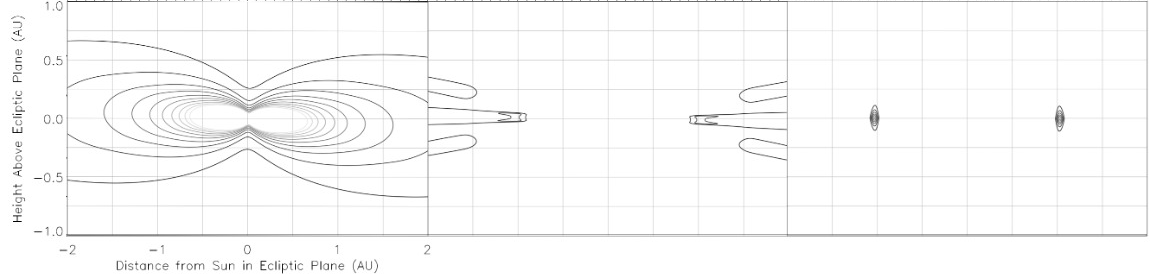
\includegraphics[width=1.0\textwidth]{img/ir_dust_components.png}
 \caption{Isodensity contours of the interplanetary dust model, shown at a plane perpendicular to the ecliptic. F.l.t.r.: the dust cloud, dust bands, and the circumsolar ring. Units of the contours are $10^{-7} ~\mathrm{AU}^{-1}$ for the dust cloud, and $0.125\cdot10^{-7} ~\mathrm{AU}^{-1}$ for the bands and ring (\cite{IRDust}).}
 \label{fig:irdustcontributions}
\end{figure}

The combined density model is shown in \autoref{fig:irdustcombined}. As can be seen, the dust cloud is the largest contributor to the density of the dust cloud. With the density and temperature components known, the infrared background due to the interplanetary dust can be modelled. The only factor that needs to be added to this is the direct thermal radiation from the Sun, which can be obtained directly from Planck's law. \\

\begin{figure}[htbp]
 \centering
 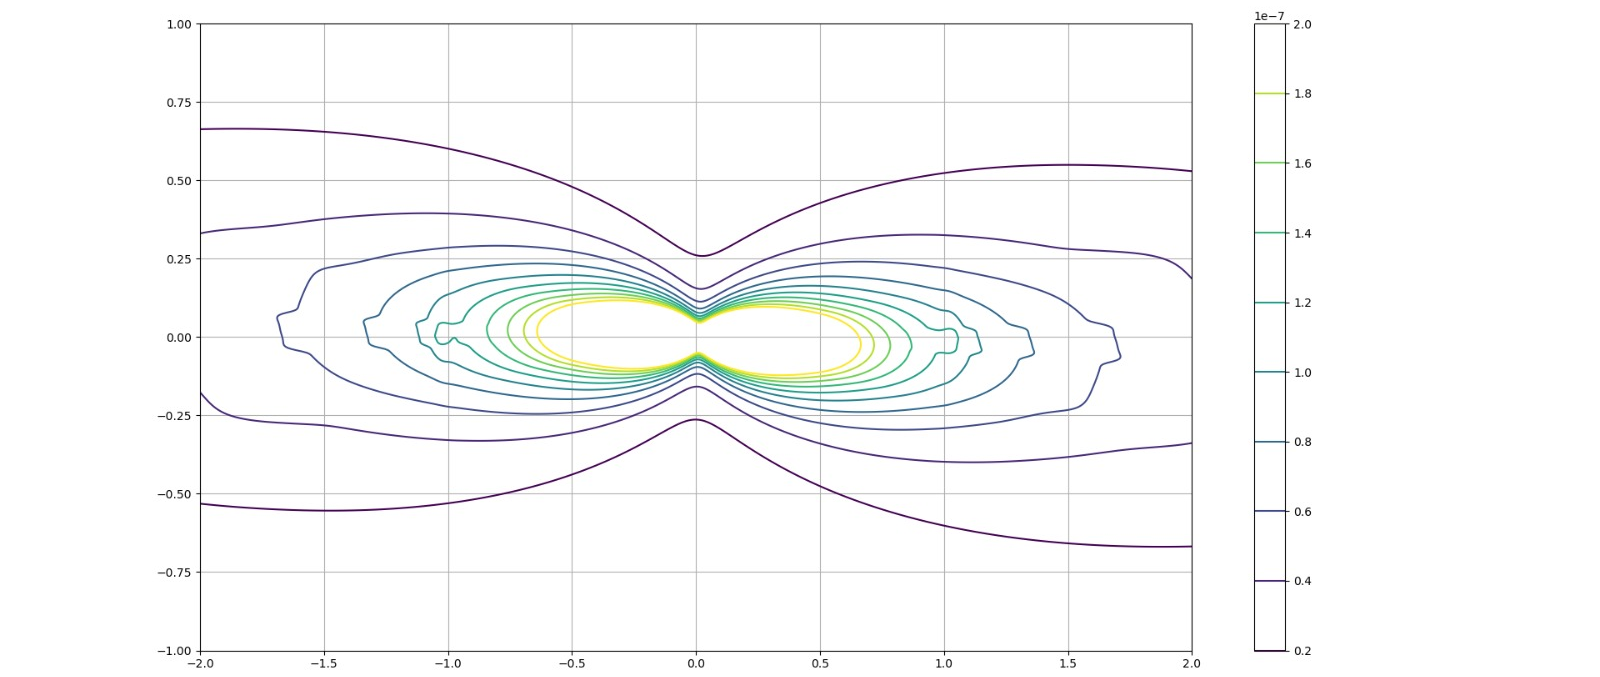
\includegraphics[width=0.6\textwidth]{img/ir_dust_combined.png}
 \caption{Combined isodensity contour of the interplanetary dust in a plane perpendicular to the ecliptic (\cite{IRDust}).}
 \label{fig:irdustcombined}
\end{figure}

Combining all these components and performing the integration leads to the full contribution as a result of Solar radiation and interplanetary dust. An illustration of the signal can be seen in \autoref{fig:solartirbackground}. The contribution from the Sun, and the hot dust near the Sun, is the most important source. However, there is still a sizeable flux originating in the interplanetary dust throughout the Solar system.\\

\begin{figure}[htbp]
 \centering
 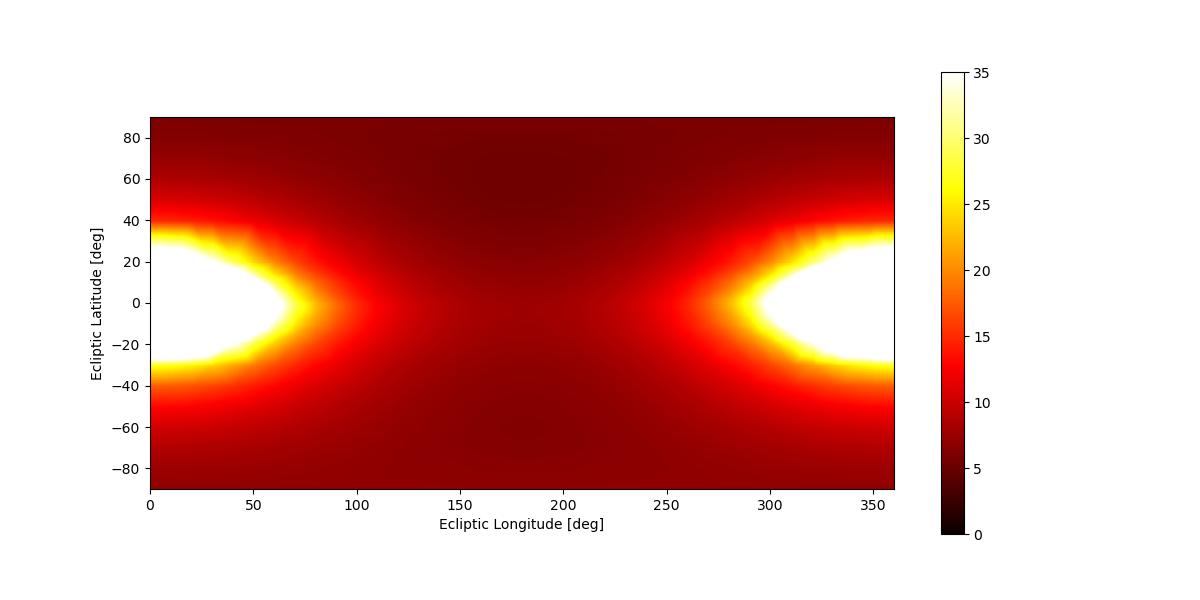
\includegraphics[width=1.0\textwidth]{img/background_tir_zodiac.png}
 \caption{Contribution of light from the Sun to the background signal in thermal infrared, in the body-fixed reference frame $b$, as seen from a spacecraft located at (-1, 0, 0) AU in the heliocentric frame $h$. Units are Megajansky per steradian, $1 \mathrm{MJy}{sr}^{-1} = 10^{-21} \mathrm{W}\mathrm{m}^{-2}\mathrm{Hz}^{-1}\mathrm{sr}^{-1}$, and the scale is clipped at $35 ~\mathrm{MJy}{sr}^{-1}$ for clarity.}
 \label{fig:solartirbackground}
\end{figure}

On the other hand, the background signal in the visual spectrum is more readily available. As it can be quickly and repeatedly measured from the surface of the Earth, early measurements of this signal exist. The components of the visual light background signal are tabulated by \cite{LightOfTheNightSky}, using data obtained from measurements. The resulting contribution from the Sun and Sunlight reflected off of interplanetary dust can be seen in \autoref{fig:solarvisbackground}. Next to the obvious contribution of the Sun and zodiacal light, the phenomenon of gegenschein can be observed in the middle of the plot. Although this is the point where target asteroids are at their brightest, it is also a point of increased background flux. The values as tabulated by \cite{LightOfTheNightSky} are only valid at a distance from the Sun of 1 AU. \cite{SkyBrightness} offer a correction factor to obtain the flux $F$ for changing heliocentric distance of the observer $R$ from the flux at 1 AU $F_{1~\mathrm{AU}}$ as follows:
\begin{equation}
 F(R) = F_{1~\mathrm{AU}}R^{-2.3}
 \label{eq:sunscale}
\end{equation}
This correction factor accounts for both the approximate decrease in interplanetary dust density when moving away from the Sun, as well as the decrease in solar flux. With these components, the Sun-dependent portion of the background signal is fully available for modelling. \\

\begin{figure}[htbp]
 \centering
 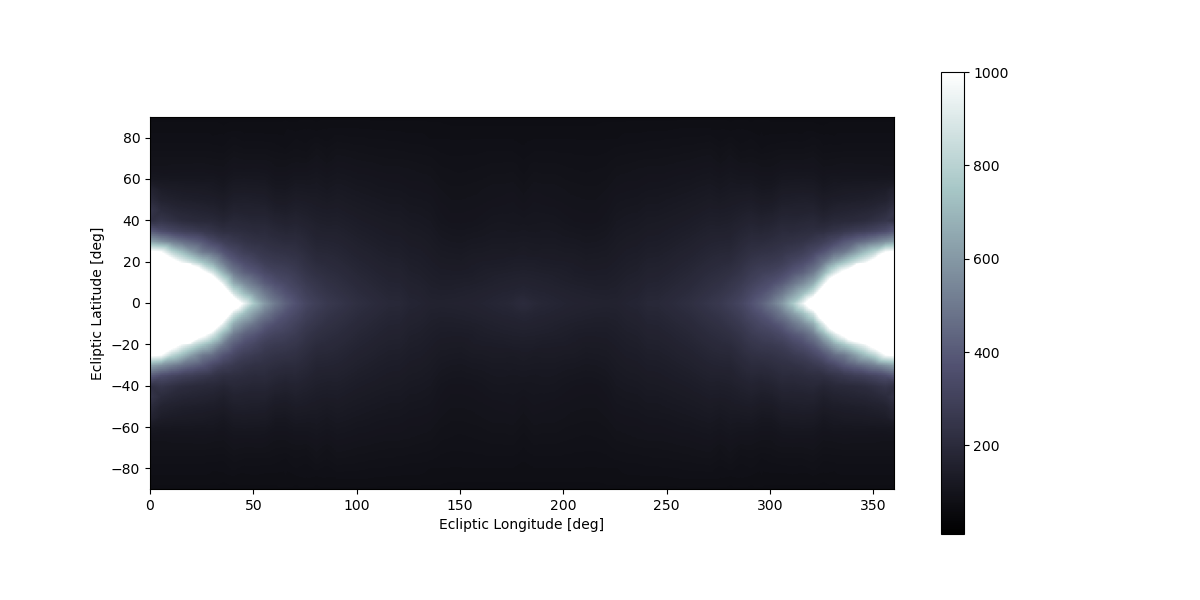
\includegraphics[width=1.0\textwidth]{img/background_vis_zodiac.png}
 \caption{Contribution of light from the Sun to the background signal in the visual spectrum, in the body-fixed reference frame $b$, as seen from a spacecraft located at (-1, 0, 0) AU in the heliocentric frame $h$. Units are $S10_\odot$ or solar-type stars of 10th magnitude per square degree. $1S10_\odot = 9.00\mathrm{W}\mathrm{m}^{-2}\mathrm{sr}^{-1}$. The scale is clipped at $1000 S10_\odot$ for clarity.}
 \label{fig:solarvisbackground}
\end{figure}


\subsection{Milky Way and Diffuse Starlight}

For the background signal originating from the Milky Way and other diffuse starlight, similar models exist for both the thermal and infrared and the visual light spectrum. By subtraction of the signal from the Sun, zodiacal light and gegenschein, the remaining portion of the background signal could be attributed to this component. The resulting models from \cite{IRDust} and \cite{LightOfTheNightSky} are shown in \autoref{fig:starstirbackground} and \autoref{fig:starsvisbackground}, respectively. Due to the research being more modern, and more computer and data storage resources being available at the time, the thermal infrared background model can be seen to be more detailed than the visual light spectrum model. However, other similarities, such as the light from the galactic core around $l_b = 270^\circ$ can be observed in both. Lastly, note that while the diffuse background starlight generally has a lesser magnitude than the emission and reflection of the interplantary dust, the Milky Way is brighter than the interplanetary dust in both spectra and thus warrants inclusion into the model. \\

\begin{figure}[htbp]
 \centering
 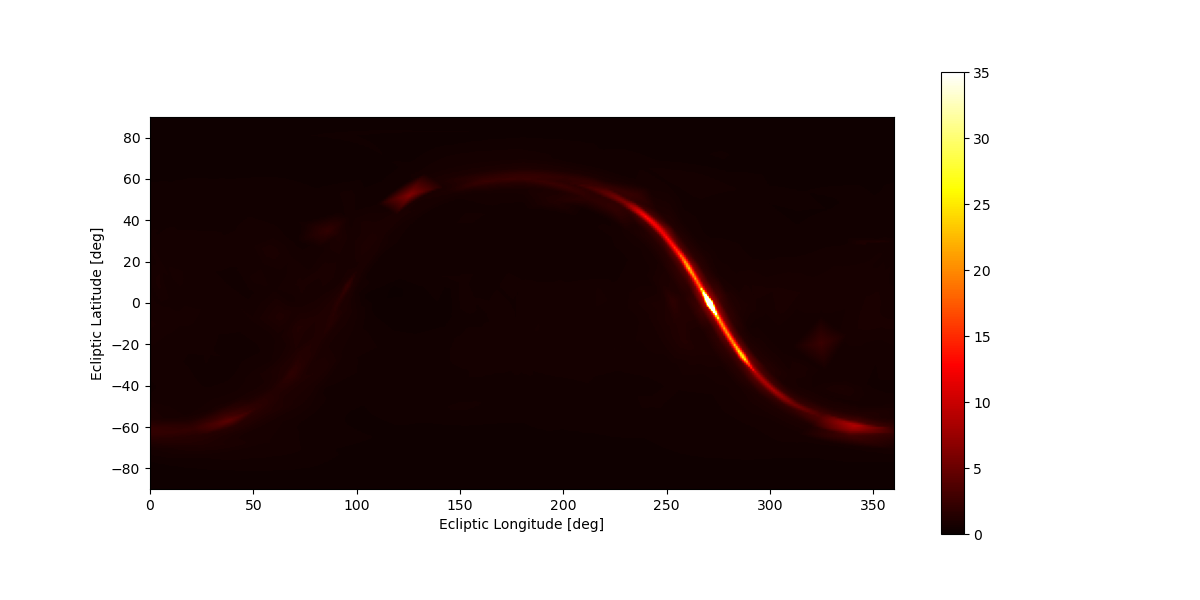
\includegraphics[width=1.0\textwidth]{img/background_tir_stars.png}
 \caption{Contribution of light from the Milky Way and diffuse starlight to the background signal in thermal infrared, in the body-fixed inertial frame $b$. Units are Megajansky per steradian, $1 \mathrm{MJy}{sr}^{-1} = 10^{-21} \mathrm{W}\mathrm{m}^{-2}\mathrm{Hz}^{-1}\mathrm{sr}^{-1}$, and the scale is clipped at $35 \mathrm{MJy}{sr}^{-1}$ for clarity.}
 \label{fig:starstirbackground}
\end{figure}

A final note is to be made about individual stars: readers who occassionally glance at the night sky are undoubtedly familiar with the fact that numerous stars outshine the diffuse background, making them appear as individual, distinct points. Naturally, these point will also appear in images taken of the sky. Similarly, large features such as distant galaxies or nebulae will contribute higher concentrations of background signal. However, as these objects are essentially fixed with regards to the movement and timescale of human surveying efforts, they have been extensively catalogued. Therefore, treatment of the signal from these objects is a fairly straightforward and well-understood process (see \cite{StarRemoval} for a thorough explanation). Even if an NEA was to pass in front of such a source, as the mean signal of the source is known, the contribution of the target can still be extracted. Therefore, it is not required to include these objects in the analysis explicitly: their effect is included in the resulting Poisson noise from the background signal.

\begin{figure}[htbp]
 \centering
 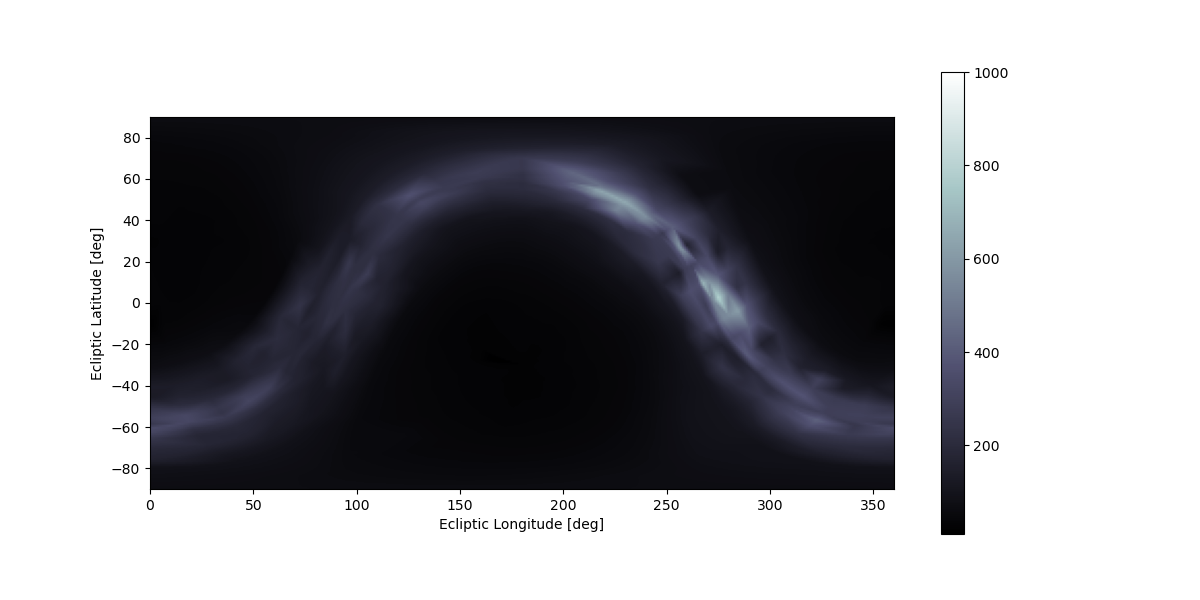
\includegraphics[width=1.0\textwidth]{img/background_vis_stars.png}
 \caption{Contribution of light from the Milky Way and diffuse starlight to the background signal in the visual spectrum, in the body-fixed inertial frame $b$. Units are $S10_\odot$ or solar-type stars of 10th magnitude per square degree. $1S10_\odot = 9.00\mathrm{W}\mathrm{m}^{-2}\mathrm{sr}^{-1}$. The scale is clipped at $1000 S10_\odot$ for clarity.}
 \label{fig:starsvisbackground}
\end{figure}


\section{Target Signal}
\label{sec:modelling_target}
In addition to modelling the background signal, the target signal has to be modelled. Although in reality the radiation emitted or reflected by an asteroid is dependent on many factors, including, but not necessarily limited to, its size, surface composition, shape, temperature and rotational motion, models exist which provide good approximations. As the asteroid population model from \cite{GranvikPopulation} gives a distribution of absolute magnitudes, the starting point of these models will also be the asteroids absolute magnitude, along with the position of the asteroid and the spacecraft relative to the Sun. \\

Firstly, for determining the emission of an asteroid in the thermal infrared, several models have been constructed in recent years. The original model for asteroids in thermal infrared is provided in the work of \cite{AsteroidSTM}. However, more recently \cite{AsteroidNEATM} have given an updated model of the thermal emissions of asteroids, and therefore their Near-Earth Asteroid Thermal Model (NEATM) is considered the standard at time of writing. \\

The NEATM assumes asteroids to be spherical, nonrotating bodies in thermal equilibrium with the radiation emitted by the Sun. The night side of the asteroid is assumed to have a temperature of $0~K$. The equilibrium temperature is modelled as follows:
\begin{align}
 T(\phi) &= \begin{cases}
            T(0) \cos ^{1/4} \phi;& \phi < 90^\circ \\
            0;& \phi \geq 90^\circ
           \end{cases} \\
T(0) &= \left[(1-A)F_{\odot}/(\eta \epsilon \sigma)\right]^{1/4}
\end{align}
With $\phi$ the angular distance from the subsolar point, $A$ the bond albedo, $F_{\odot}$ the incident solar flux, $\epsilon$ the emissivity, $\sigma$ the Stefan-Boltzmann constant and $\eta$ the so-called \textit{beaming parameter}, a correction factor for the emission dependent on the non-sphericalness of the surface, which can be calibrated from observations. For the NEATM, this value is set to $\eta = 1.22$.\\

With the temperature distribution known, the emission can be determined through integration of Planck's law over the visible hemisphere. For this, the size of the asteroid needs to be determined, which can be done using \autoref{eq:asteroidsize}. Estimation of this albedo using current data is difficult, and therefore the previously mentioned value of $p_v = 0.14$ is assumed. Of course, this calculation is sensitive to the assumed value of the albedo. A future system utilizing both visual and thermal infrared measurements could use this dependancy on albedo to calculate the asteroid's size \textit{and} albedo, instead of only the absolute magnitude by comparing the target's signal in the visual spectrum (which is dependent on size and albedo), to the signal in the thermal infrared (which is only dependent on the size). This might lead to better estimates of these values in the future.\\

Calculation of the target signal in the visual spectrum is more straightforward, as no integration is needed; a simple phase equation is readily available to obtain the apparent visual magnitude $V$, as detailed by \cite{2003NEOSDT}:
\begin{align}
 V &= H + 5 \log r \Delta - 2.5 \log \left[ (0.85) \Phi_1 + 0.15 \Phi_2 \right] \\
 \Phi_1 &= e^{-3.33\left(\tan \frac{\alpha}{2} \right)^{0.63}} \\
 \Phi_2 &= e^{-1.87\left(\tan \frac{\alpha}{2} \right)^{1.22}}
\end{align}
For solar elongations less than 60 degrees, \cite{2003NEOSDT} suggest using a modified equation instead:
\begin{equation}
 V = H + 5 \log r \Delta + 5.03 - 10.373 \log (\pi - \alpha)
\end{equation}
In these equations, $H$ is the absolute magnitude, $\alpha$ is the solar phase angle, $r$ is the distance from the Sun to the target and $\Delta$ is the distance from the observer to the target. By definition, the ratio between a flux $F_2$ and a reference flux $F_1$ can be determined from the difference in their apparent magnitude $\Delta V$:
\begin{equation}
 \frac{F_2}{F_1} = 100^{\frac{\Delta V}{5}}
\end{equation}
As the Sun has an apparent magnitude of $V_\odot = -26.74$, and a flux of $F_\odot = 1361 \mathrm{W}\mathrm{m}^{-2}$ at 1 AU, the visual flux of the target $F_t$ can be calculated from its apparent magnitude $V_t$ as follows:
\begin{equation}
 F_t = F_\odot 100^{\frac{-26.74 - V_t}{5}}
\end{equation}
It is here where part of the difficulty of detecting very small NEAs becomes apparent: relative to a $D = 3.5 \mathrm{km}$ asteroid ($V \approx 15$), a $D = 350 \mathrm{m}$ asteroid ($V \approx 20$) only results in 1/100th of the flux, and a $D = 35 \mathrm{m}$ asteroid ($V \approx 25$) will only give off 1/10,000th of the flux in both spectra. Note also that there is no \textit{inherent} advantage to either method in detecting small NEAs when considering the target signal. However, the thermal infrared background signal is relatively smaller relative to the target signal (\cite{2003NEOSDT}).

\section{Hardware Properties and Signal-to-Noise Ratio}
\label{sec:modelling_hardware_SNR}

In addition to the signal properties, the hardware used to image the target is also of interest. Some of the properties of the hardware can then be used to compute the signal-to-noise ratio (SNR) of the target, and several other properties will be used in the next section to determine the search strategy and cadence. \cite{2017NEOSDT} gives a description of representative hardware for current and upcoming space survey telescopes. The overview can be seen in \autoref{tab:hardwareproperties}. For the thermal infrared, a HgCdTe detector is utilized, for the visual light a silicon CCD. \\

\begin{table}[htbp]
\centering
\caption{Representative hardware properties for space-based survey telescopes. (\cite{2017NEOSDT})}
\label{tab:hardwareproperties}
\begin{tabular}{ll|ll}
\textbf{Parameter}        &  & \textbf{Thermal Infrared} & \textbf{Visual Light} \\ \hline
Aperture &{[}m{]}            & 0.5                       & 0.5                   \\
Field of view &{[}deg{]}     & 1.7 x 7.13                & 10.6 x 5.3            \\
Bandpass &{[}$\mu$m{]}       & 6 - 10                    & 0.4 - 1.0             \\
Integration time &{[}s{]}    & 150                       & 24                    \\
Quantum efficiency &{[}\%{]} & 65                        & 88                    \\
Dark current &{[}e-/s{]}     & 1                         & 0.00055               \\
Read noise &{[}e-{]}         & 22                        & 4
\end{tabular}
\end{table}

Two important observations should be made from the data in \autoref{tab:hardwareproperties}. Firstly, the visual light system has better specifications with regards to noise and quantum efficiency. This is due to the more advanced level of technology in CCD development compared to thermal infrared detectors. Secondly, the square angle subtended by the visual light sensor is almost five times as large as the thermal infrared sensor, and the required integration time is less than one sixth. The former factor is also due to discrepancies in technological development, the latter is a result of the weaker signal in the thermal infrared band. Together, these factors result in a sizeable decrease in survey cadence, which will be discussed in the next section. A last factor which is not shown in the table is the requirement for thermal infrared telescopes to be cooled to very low temperatures, to avoid the heat of the telescope itself interfering with the measurements. Visual light telescopes are not hindered much by their own temperature, as spacecraft at normal operating temperatures emit very little visible light. \\

The signal-to-noise ratio of the observation can then be calculated by dividing the signal in $e^-$ by the root-sum-square of the noise terms, assuming the noise terms to be independent (\cite{DetectionAndTracking}):
\begin{equation}
 SNR = \frac{S_t}{\sqrt{S_t + S_b + D + R^2}}
\end{equation}
The target signal $S_t$ and background signal $S_b$ can be calculated from the flux $F$ as follows (\cite{DetectionAndTracking}):
\begin{align}
 S_t &= \frac{1}{hc}A \tau k_f Q_e F_t \\
 S_b &= \frac{1}{hc}A \tau Q_e F_b
\end{align}
Here, $A$ is the telescope aperture, $\tau$ the integration time of the image, $k_f$ is the \textit{straddle factor}, a correction factor for the diffraction of a point source ($k_f \approx 0.9$), $Q_e$ the quantum efficiency, and $h$ and $c$ the Planck constant and speed of light, respectively. The background flux is obtained by summation of the components described in \autoref{sec:modelling_background} in the direction of the target; the implementation of calculation of the target flux is described in the next chapter. The noise terms in the SNR equation are:
\begin{itemize}
 \item $\sqrt{S_t}$: the Poisson noise of the target signal.
 \item $\sqrt{S_b}$: the Poisson noise of the background signal. Note that the background signal itself can be subtracted fairly easy, and thus only the Poisson term has to be considered (see \cite{StarRemoval}).
 \item $\sqrt{D}$: the Poisson term of the dark current noise. The mean dark current can be removed through proper sensor calibration (see \cite{OpNav}).
 \item $\sqrt{R}$: the readout noise.
\end{itemize}

Thus, the SNR of every target can be calculated at any point in time from any telescope in space in both the thermal infrared and visual light spectrum.

\section{Search Strategy and Cadence}
\label{sec:modelling_cadence}
Next, it is important to consider how the telescope will conduct the survey. Of course, a telescope can not view in all directions simultaneously. Very little literature exists on setup and optimization of such search strategies. \cite{Cadence} provides some guidance based on the search strategy for the NEOCam mission. Essentially, the telescope performs a grid-like search, from north to south and west to east. Each section of the sky is revisited four times in a short time to allow for determining the direction of motion of targets, which aids in the precision of orbital determination. Thus, the number of images required to image the entire sky once, $n_{images}$ is approximately four times the solid angle of a sphere $\Omega = \frac{360^2}{\pi} = 41253\mathrm{deg}^2$, divided by the solid angle subtended by the image sensor's field of view $\Theta$:
\begin{equation}
 n_{images} = 4\frac{41253\mathrm{deg}^2}{\Theta}
\end{equation}
The time required per image $t_{image}$ is the summation of three terms: the integration time $\tau$, the settle time $t_{settle}$, and the slew time $t_{slew}$, where the latter can be approximated conservatively by taking the larger of the two dimensions of the image sensor, $\theta_1$, and dividing it by the slew rate $\dot{\theta}$:
\begin{equation}
 t_{image} = \tau + \frac{\theta_1}{\dot{\theta}} + t_{settle}
\end{equation}
The survey cadence (the time required to do one survey cycle of imaging the entire sky; i.e. a survey cadence of ten implies the telescope images the entire sky every ten days) is then given by:
\begin{equation}
 T_{survey} = n_{images}t_{image}
\end{equation}

From the previously stated hardware properties of the visual light telescope in \autoref{tab:hardwareproperties}, and assuming a slew rate of $\dot{\theta} = 0.5^\circ\mathrm{s}^{-1}$ and a settle time of $t_{settle} = 10 \mathrm{s}$ the following values are obtained:
\begin{align}
 \Theta &= 10.6 * 5.3 = 56.18\mathrm{deg}^2 \\
 \theta_1 &= \mathrm{max}(10.6, 5.3) = 10.6 \mathrm{deg} \\
 \tau &= 24 \mathrm{s} \\
 t_{slew} &= \frac{10.6}{0.5} = 21.2 \mathrm{s} \\
 t_{settle} &= 10 \mathrm{s} \\
\end{align}
Therefore:
\begin{align}
 n_{images} &= 4\frac{41253}{56.18} = 2938~\mathrm{images~per~survey~cycle}\\
 t_{image} &= 24 + 21.2 + 10 = 55.2~\mathrm{seconds~per~image}\\
 T_{survey} &= 2938 * 55.2 = 162,177.6~\mathrm{seconds~per~survey} \approx 1.88~\mathrm{days~per~survey}
\end{align}

Which, at a duty cycle of just over 90\% represents a fair assumption of the visual survey cadence of 2 days. Similarly, a survey cadence of 21 days was calculated for the thermal infrared system. Note that, as already alluded to in the previous section, the thermal infrared system has a far slower survey cadence, which will hinder the identification performance. Therefore, no system can yet be said to be superior: the thermal infrared system benefits from increased imaging performance, but a worse survey cadence.

\section{Detection and Identification}
\label{sec:modelling_identification}

From the signal-to-noise ratio, detection and identification can finally be established. Firstly, detection of the signal from the noise. As described by \cite{2017NEOSDT}, detection in processed images is a probabilistic process: At low SNR (SNR < 1), while detection is possible, the detection should be rejected because the probability of false detections becomes too high. Conversely, at high SNR (SNR > 5), detection becomes almost certain: the risk of false positives is so small that detection can be established aggressively. Modelling the process by a normal distribution allows for the intermittent range of SNR to be approximated by an integrated Gaussian. This distribution can be seen in \autoref{fig:snrgraph}. \\

\begin{figure}[htbp]
 \centering
 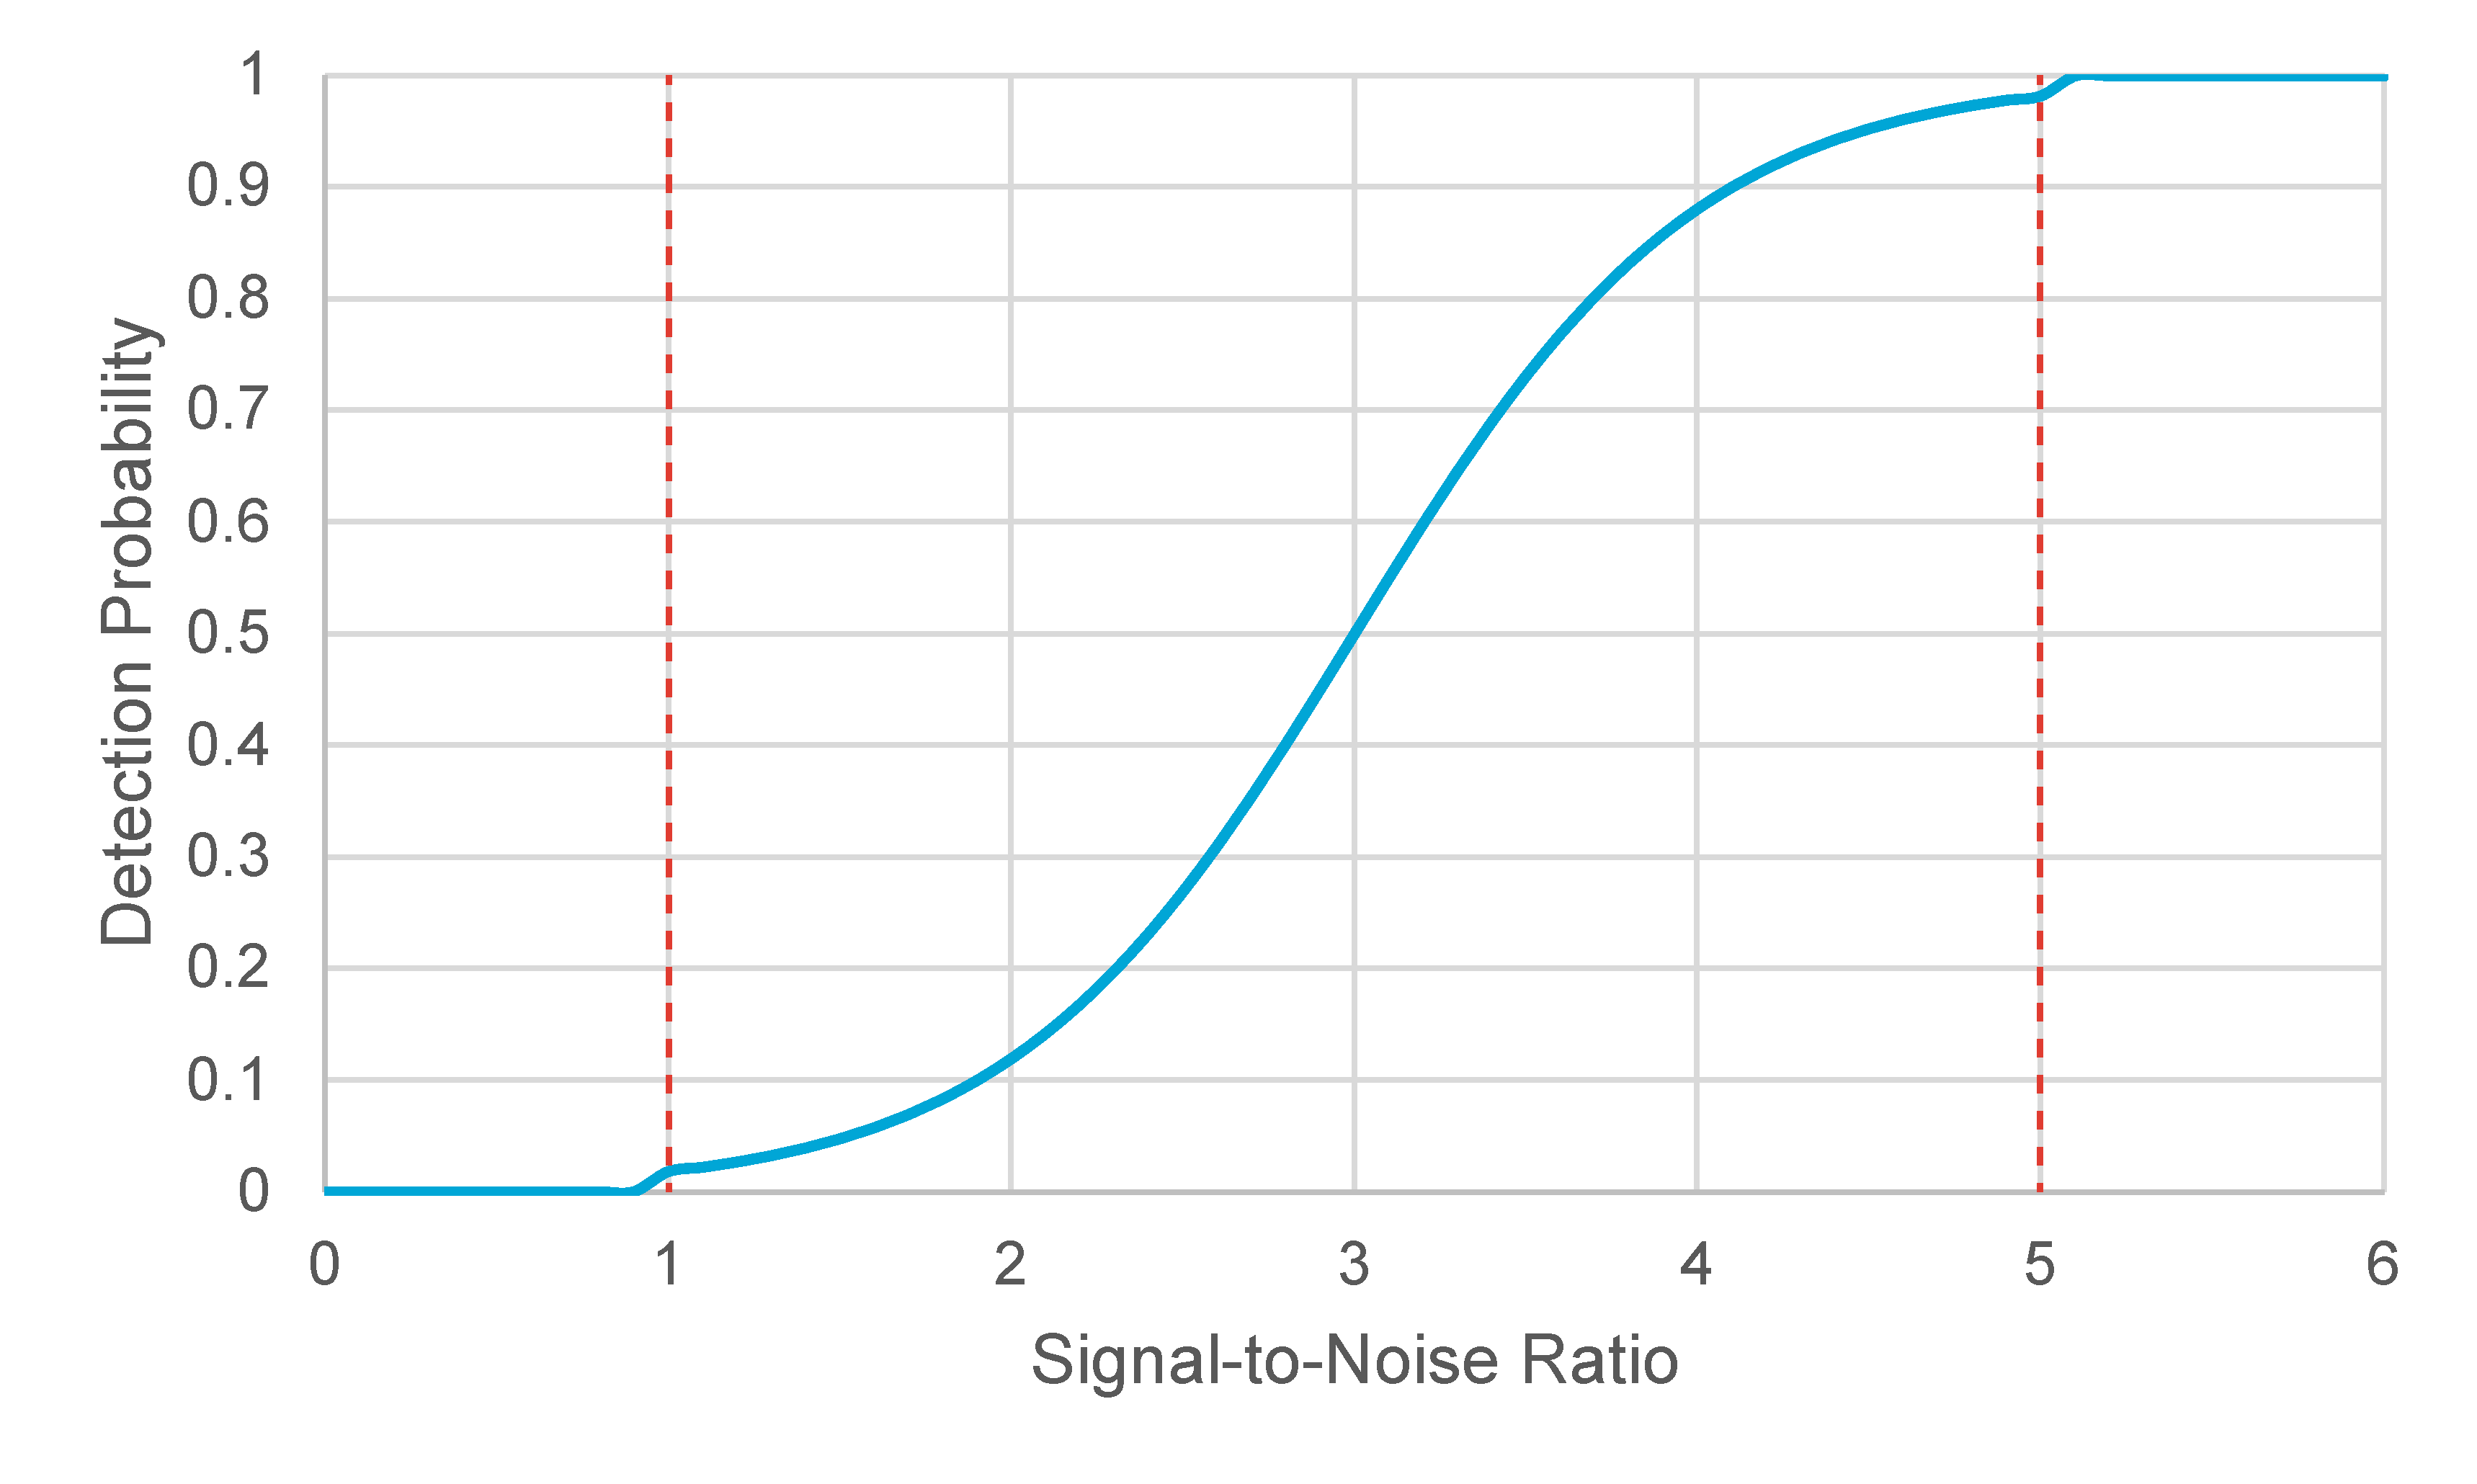
\includegraphics[width=0.7\textwidth]{img/snr_graph.pdf}
 \caption{Detection probability as a function of signal-to-noise ratio according to an integrated Gaussian. The function is truncated to 0 at SNR < 1, and to 1 at SNR > 5: at very low SNR, detection should be rejected as the possibility of false positives becomes too high; at very high SNR, the risk of false positives becomes so small that detection essentially becomes a certainty.}
 \label{fig:snrgraph}
\end{figure}

The process of identification is slightly more complicated. In essence, the process of solving for the orbit of a target asteroid using a single telescope uses Gauss' method, to obtain an orbit from three sets of angular measurements and the time between these. When multiple spacecraft are used and trangulation can be performed, two sets of positions and the time between these is enough to solve for the orbit, per Lambert's problem (see e.g. \cite{Curtis} for a thorough treatment of both methods). Theoretically, the time between these observations does not matter much, as long as the period is long enough to ensure that the curvature of the arc is larger than the uncertainty in the measurement (\cite{OpNav}). However in practice, the problem of \textit{linking} the observations arises: how does the system know that two observations spaced far apart in time belong to the same object? Currently, in practice, this results in a maximum time between subsequent observations ranging from 30 and 90 days (\cite{DetectionAndTracking}, \cite{2017NEOSDT}). However, it is expected that the resulting limit will be located more towards the maximum due to new techniques such as those presented by \cite{ShortArcs} and subsequent papers.\\

However, these methods rely on data being available throughout the system. It is currently unclear what data would need to be shared precisely, as no multi-spacecraft surveying systems have been researched to that level of detail to date. However, as \cite{2017NEOSDT} state, communication of survey results will be a point of attention for all deep-space surveying missions, not just multi-spacecraft ones, and an advanced communication system along with on-board data processing will be required. Luckily, modern techniques such as machine learning are being used to find computationally unintensive and simple solutions to the image processing pipeline (see, e.g., \cite{AIImage}). Therefore, this point will be considered to be out of scope of the research presented in this report. \\

With the detection and identification treated, a full overview has thus been presented of the process from obtaining the signal of both background and target, calculating the resulting SNR, and establishing detection and identification of NEAs. In the next chapter, implementation of these methods will be discussed.
